\documentclass[6008notes.tex]{subfiles}
\begin{document}
\graphicspath{ {images/infbayes/} }

\section{Inference with Bayes' Theorem for Random Variables}

\subsection{The Product Rule for Random Variables (Also Called the Chain Rule)}

In many real world problems, we aren't given what the joint distribution of two random variables is although we might be given other information from which we can compute the joint distribution. Often times, we can compute out the joint distribution using what's called the product rule (often also called the chain rule). This is precisely the random variable version of the product rule for events.

As we saw from before, we were able to derive Bayes' theorem for events using the product rule for events: $\mathbb {P}(\mathcal{A} \cap \mathcal{B}) = \mathbb {P}(\mathcal{A}) \mathbb {P}(\mathcal{B} \mid \mathcal{A})$. The random variable version of the product rule is derived just like the event version of the product rule, by rearranging the equation for the definition of conditional probability. For two random variables $X$ and $Y$ (that take on values in sets $\mathcal{X}$ and $\mathcal{Y}$ respectively), the product rule for random variables says that

{\centering$p_{X,Y}(x,y)=p_{Y}(y)p_{X\mid Y}(x\mid y)\qquad \text {for all }x\in \mathcal{X},y\in \mathcal{Y}\text { such that }p_{Y}(y)>0.$ \par}
 
\paragraph{Interpretation:} If we have the probability table for $Y$, and separately the probability table for $X$ conditioned on $Y$, then we can come up with the joint probability table (i.e., the joint distribution) of $X$ and $Y$.

What happens when $p_{Y}(y)=0$? Even though $p_{X\mid Y}(x\mid y)$ isn't defined in this case, one can readily show that $p_{X,Y}(x,y)=0$ when $p_{Y}(y)=0$.

To see this, think about what is happening computationally: Remember how $p_Y(y)$ is computed from joint probability table $p_{X,Y}$? In particular, we have $p_{Y}(y)=\sum _{x}p_{X,Y}(x,y)$, so $p_Y(y)$ is the sum of either a row or a column in the joint probability table (whether it's a row or column just depends on how you write out the table and which random variable is along which axis along rows or columns). So if $p_{Y}(y)=0$, it must mean that the individual elements being summed are 0 (since the numbers we're summing up are nonnegative).

We can formalize this intuition with a proof:

\paragraph{Claim:} Suppose that random variables $X$ and $Y$ have joint probability table $p_{X,Y}$ and take on values in sets $\mathcal{X}$ and $\mathcal{Y}$ respectively. Suppose that for a specific choice of $y\in \mathcal{Y}$, we have $p_{Y}(y)=0$. Then

{\centering$p_{X,Y}(x,y)=0\qquad \text {for all }x\in \mathcal{X}.$ \par}
 
\paragraph{Proof:} Let $y\in \mathcal{Y}$ satisfy $p_{Y}(y)=0$. Recall that we relate marginal distribution $p_Y$ to joint distribution $p_{X,Y}$ via marginalization:

{\centering$0=p_{Y}(y)=\sum _{x\in \mathcal{X}}p_{X,Y}(x,y).$ \par}
 
Next, we use a crucial mathematical observation: If a sum of nonnegative numbers (such as probabilities) equals 0, then each of the numbers being summed up must also be 0 (otherwise, the sum would be positive!). Hence, it must be that each number being added up in the right-hand side sum is 0, i.e.,

{\centering$p_{X,Y}(x,y)=0\qquad \text {for all }x\in \mathcal{X}.$ \par}
 
This completes the proof. $\square$

Thus, in general:

\begin{eqnarray*}
p_{X,Y}(x,y)
&=&
\begin{cases}
p_{Y}(y)p_{X\mid Y}(x\mid y) & \text{if }p_{Y}(y)>0,\\
0 & \text{if }p_{Y}(y)=0.
\end{cases}
\end{eqnarray*}

\paragraph{Important convention for this course:} For notational convenience, throughout this course, we will often just write $p_{X,Y}(x,y)=p_{Y}(y)p_{X\mid Y}(x\mid y)$ with the understanding that if $p_{Y}(y)=0$, even though $p_{X\mid Y}(x\mid y)$ is not actually defined, $p_{X,Y}(x,y)$ just evalutes to 0 anyways.

\paragraph{The product rule is symmetric:} We can use the definition of conditional probability with $X$ and $Y$ swapped, and rearranging factors, we get:

{\centering$p_{X,Y}(x,y)=p_{X}(x)p_{Y\mid X}(y\mid x)\qquad \text {for all }x\in \mathcal{X},y\in \mathcal{Y}\text { such that }p_{X}(x)>0,$ \par}
 
and so similarly we could show that

\begin{eqnarray*}
p_{X,Y}(x,y)
&=&
\begin{cases}
p_{X}(x)p_{Y\mid X}(y\mid x) & \text{if }p_{X}(x)>0,\\
0 & \text{if }p_{X}(x)=0.
\end{cases}
\end{eqnarray*}

Again for notational convenience, we'll typically just write $p_{X,Y}(x,y)=p_{X}(x)p_{Y\mid X}(y\mid x)$ with the understanding that the expression is 0 when $p_{Y}(y)=0$.

\paragraph{Interpretation:} If we're given the probability table for $X$ and, separately, the probability table for $Y$ conditioned on $X$, then we can come up with the joint probability table for $X$ and $Y$.

Importantly, for any two jointly distributed random variables $X$ and $Y$, the product rule is always true, without making any further assumptions! Also, as a recurring theme that we'll see later on as well, we are decomposing the joint distribution into the product of factors (in this case, the product of two factors).

\paragraph{Many random variables:} If we have many random variables, say, $X_1$, $X_2$, up to $X_N$ where $N$ is not a random variable but is a fixed constant, then we have

\begin{eqnarray*}
&&p_{X_1, X_2, \dots ,X_N}(x_1, x_2, \dots, x_N) \\
&&=
  p_{X_1}(x_1)
  p_{X_2 \mid X_1}(x_2 \mid x_1)
  p_{X_3 \mid X_1, X_2}(x_3 \mid x_1, x_2) \\
  % p_{X_4 \mid X_1, X_2, X_3}(x_4 \mid x_1, x_2, x_3)
&&\quad
  \cdots
  p_{X_N \mid X_1, X_2, \dots, X_{N-1}}(x_N \mid x_1, x_2, \dots, x_{N-1}).
\end{eqnarray*}

Again, we write this to mean that this holds for every possible choice of $x_1, x_2, \dots , x_ N$ for which we never condition on a zero probability event. Note that the above factorization always holds without additional assumptions on the distribution of $X_1, X_2, \dots , X_ N$.

Note that the product rule could be applied in arbtirary orderings. In the above factorization, you could think of it as introducing random variable $X_1$ first, and then $X_2$, and then $X_3$, etc. Each time we introduce another random variable, we have to condition on all the random variables that have already been introduced.

Since there are $N$ random variables, there are $N!$ different orderings in which we can write out the product rule. For example, we can think of introducing the last random variable $X_ N$ first and then going backwards until we introduce $X_1$ at the end. This yields the, also correct, factorization

\begin{eqnarray*}
&& p_{X_1, X_2, \dots ,X_N}(x_1, x_2, \dots, x_N) \\
&&=
  p_{X_N}(x_N)
  p_{X_{N-1} \mid X_N}(x_{N-1} \mid x_N)
  p_{X_{N-2} \mid X_{N-1}, X_N}(x_{N-2} \mid x_{N-1}, x_N) \\
  % p_{X_4 \mid X_1, X_2, X_3}(x_4 \mid x_1, x_2, x_3)
&&\quad
  \cdots
  p_{X_1 \mid X_2, X_3, \dots, X_N}(x_1 \mid x_2, \dots, x_N).
\end{eqnarray*}

\subsection{Bayes' Rule for Random Variables (Also Called Bayes' Theorem for Random Variables}

In inference, what we want to reason about is some unknown random variable $X$, where we get to observe some other random variable $Y$, and we have some model for how $X$ and $Y$ relate. Specifically, suppose that we have some “prior" distribution $p_X$ for $X$; this prior distribution encodes what we believe to be likely or unlikely values that $X$ takes on, before we actually have any observations. We also suppose we have a “likelihood" distribution $p_{Y\mid X}$.

After observing that $Y$ takes on a specific value $y$, our “belief" of what $X$ given $Y=y$ is now given by what's called the “posterior" distribution $p_{X\mid Y}(\cdot \mid y)$. Put another way, we keep track of a probability distribution that tells us how plausible we think different values $X$ can take on are. When we observe data $Y$ that can help us reason about $X$, we proceed to either upweight or downweight how plausible we think different values $X$ can take on are, making sure that we end up with a probability distribution giving us our updated belief of what $X$ can be.

Thus, once we have observed $Y=y$, our belief of what $X$ is changes from the prior $p_X$ to the posterior $p_{X\mid Y}(\cdot \mid y)$.

Bayes' theorem (also called Bayes' rule or Bayes' law) for random variables explicitly tells us how to compute the posterior distribution $p_{X\mid Y}(\cdot \mid y)$, i.e., how to weight each possible value that random variable $X$ can take on, once we've observed $Y=y$. Bayes' theorem is the main workhorse of numerous inference algorithms and will show up many times throughout the course.

\paragraph{Bayes' theorem:} Suppose that $y$ is a value that random variable $Y$ can take on, and $p_{Y}(y)>0$. Then

{\centering$p_{X\mid Y}(x\mid y)=\frac{p_{X}(x)p_{Y\mid X}(y\mid x)}{\sum _{ x'}p_{X}( x')p_{Y\mid X}(y\mid x')}$ \par}
 
for all values $x$ that random variable $X$ can take on.

\paragraph{Important:} Remember that $p_{X\mid Y}(\cdot \mid y)$ could be undefined but this isn't an issue since this happens precisely when $p_X(x)=0$, and we know that $p_{X,Y}(x,y)=0$ (for every $y$) whenever $p_X(x)=0$.

\paragraph{Proof:} We have

{\centering$p_{X\mid Y}(x\mid y)\overset {(a)}{=}\frac{p_{X,Y}(x,y)}{p_{Y}(y)}\overset {(b)}{=}\frac{p_{X}(x)p_{Y\mid X}(y\mid x)}{p_{Y}(y)}\overset {(c)}{=}\frac{p_{X}(x)p_{Y\mid X}(y\mid x)}{\sum _{ x'}p_{X,Y}( x',y)}\overset {(d)}{=}\frac{p_{X}(x)p_{Y\mid X}(y\mid x)}{\sum _{ x'}p_{X}( x')p_{Y\mid X}(y\mid x')},$ \par}
 
where step $(a)$ uses the definition of conditional probability (this step requires $p_Y(y)>0)$, step $(b)$ uses the product rule (recall that for notational convenience we're not separately writing out the case when $p_X(x)=0)$, step $(c)$ uses the formula for marginalization, and step $(d)$ uses the product rule (again, for notational convenience, we're not separately writing out the case when $p_X(x')=0$). $\square$

\subsection{Bayes' Theorem for Random Variables: A Computational View}

Computationally, Bayes' theorem can be thought of as a two-step procedure. Once we have observed $Y=y$:

For each value $x$ that random variable $X$ can take on, initially we believed that $X=x$ with a score of $p_X(x)$, which could be thought of as how plausible we thought ahead of time that $X=x$. However now that we have observed $Y=y$, we weight the score $p_X(x)$ by a factor $p_{Y\mid X}(y\mid x)$, so

{\centering$\text {new belief for how plausible }X=x\text { is:}\quad \alpha (x\mid y)\triangleq p_{X}(x)p_{Y\mid X}(y\mid x),$ \par}

where we have defined a new table $\alpha (\cdot \mid y)$ which is not a probability table, since when we put in the weights, the new beliefs are no longer guaranteed to sum to 1 (i.e., $\sum _{x}\alpha (x\mid y)$ might not equal 1)! $\alpha (\cdot \mid y)$ is an unnormalized posterior distribution!

Also, if $p_X(x)$ is already 0, then as we already mentioned a few times, $p_{Y\mid X}(y\mid x)$ is undefined, but this case isn't a problem: no weighting is needed since an impossible outcome stays impossible.

To make things concrete, here is an example from the medical diagnosis problem where we observe $Y=positive$:

{\centering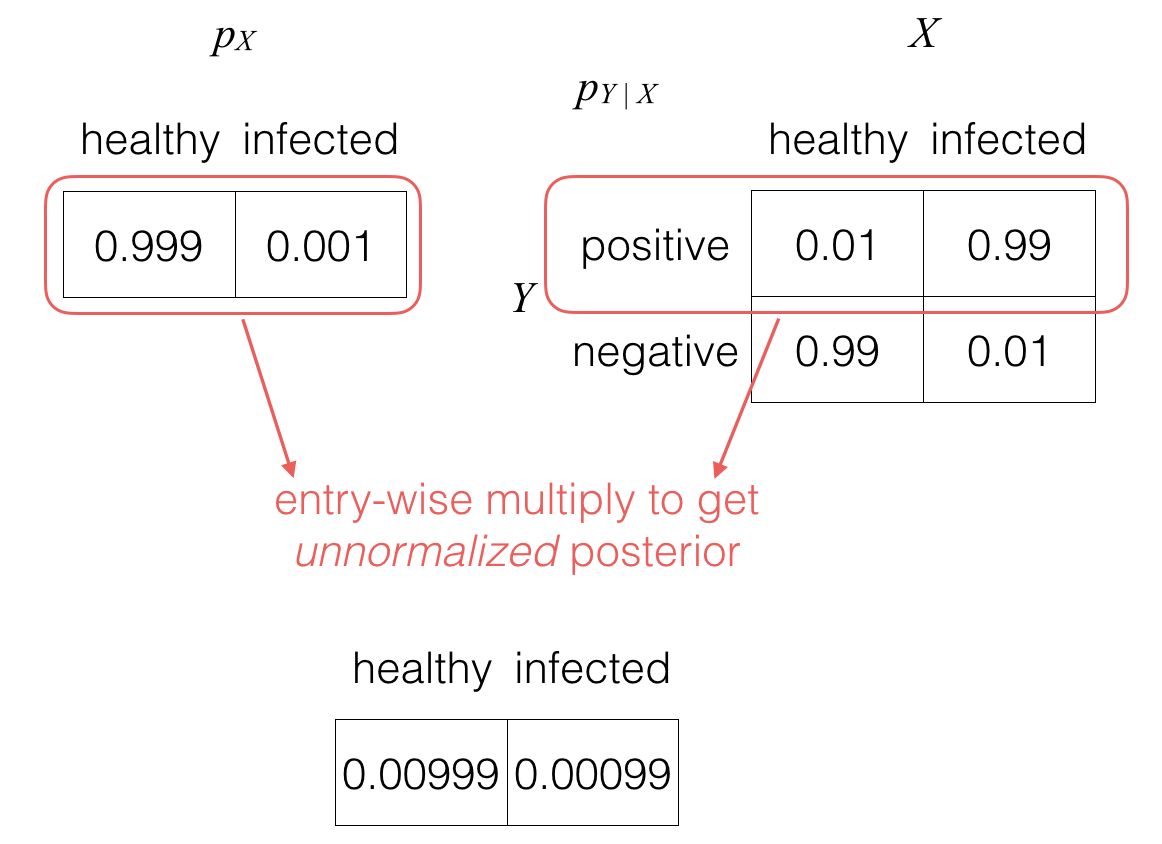
\includegraphics[scale=0.3]{images_sec-bayes-computational-view} \par}

We fix the fact that the unnormalized posterior table $\alpha (\cdot \mid y)$ isn't guaranteed to sum to 1 by renormalizing:

{\centering$p_{X\mid Y}(x\mid y)=\frac{\alpha (x\mid y)}{\sum _{ x'}\alpha ( x'\mid y)}=\frac{p_{X}(x)p_{Y\mid X}(y\mid x)}{\sum _{ x'}p_{X}( x')p_{Y\mid X}(y\mid x')}.$ \par}
 
An important note: Some times we won't actually care about doing this second renormalization step because we will only be interested in what value that $X$ takes on is more plausible relative to others; while we could always do the renormalization, if we just want to see which value of $x$ yields the highest entry in the unnormalized table $\alpha (\cdot \mid y)$, we could find this value of $x$ without renormalizing!

\subsection{Maximum A Posteriori (MAP) Estimation}

For a hidden random variable $X$ that we are inferring, and given observation $Y=y$, we have been talking about computing the posterior distribution $p_{X \mid Y}(\cdot | y)$ using Bayes' rule. The posterior is a distribution for what we are inferring. Often times, we want to report which particular value of $X$ actually achieves the highest posterior probability, i.e., the most probable value $x$ that $X$ can take on given that we have observed $Y=y$.

The value that $X$ can take on that maximizes the posterior distribution is called the \textit{maximum a posteriori} (MAP) estimate of $X$ given $Y=y$. We denote the MAP estimate by $\widehat{x}_{\text {MAP}}(y)$, where we make it clear that it depends on what the observed $y$ is. Mathematically, we write

{\centering$\widehat{x}_{\text {MAP}}(y) = \arg \max _ x p_{X \mid Y}(x | y).$ \par}
 
Note that if we didn't include the ``arg'' before the ``max'', then we would just be finding the highest posterior probability rather than which value -- or ``argument'' -- $x$ actually achieves the highest posterior probability.

In general, there could be ties, i.e., multiple values that $X$ can take on are able to achieve the best possible posterior probability.


\end{document}